\chapter{UI Overview}

In this section, the main GUI components are described, to give an overview and introduce the different workflow options.

\subfile{ui_main_window}

\section{Main Menu}

\subsection{File Menu}

Databases can be created, opened and closed using the File menu.

\begin{figure}[H]
  \center
    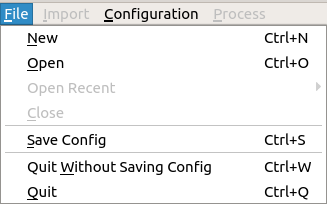
\includegraphics[width=6cm,frame]{figures/ui_file_menu.png}
  \caption{File Menu}
\end{figure}

\begin{itemize}
 \item New: Create new database file
 \item Open: Open existing database file
 \item Open Recent: Open recent existing database file
 \item Close: Close current database
 \item Save Config: Save current configuration
 \item Quit Without Saving Config: Quit application without saving configuration
 \item Quit: Quit application with saving configuration
\end{itemize}
\  \\

After a database was opened, the 'Import' menu becomes available, and the main window looks as follows:

\begin{figure}[H]
  \hspace*{-2.5cm}
    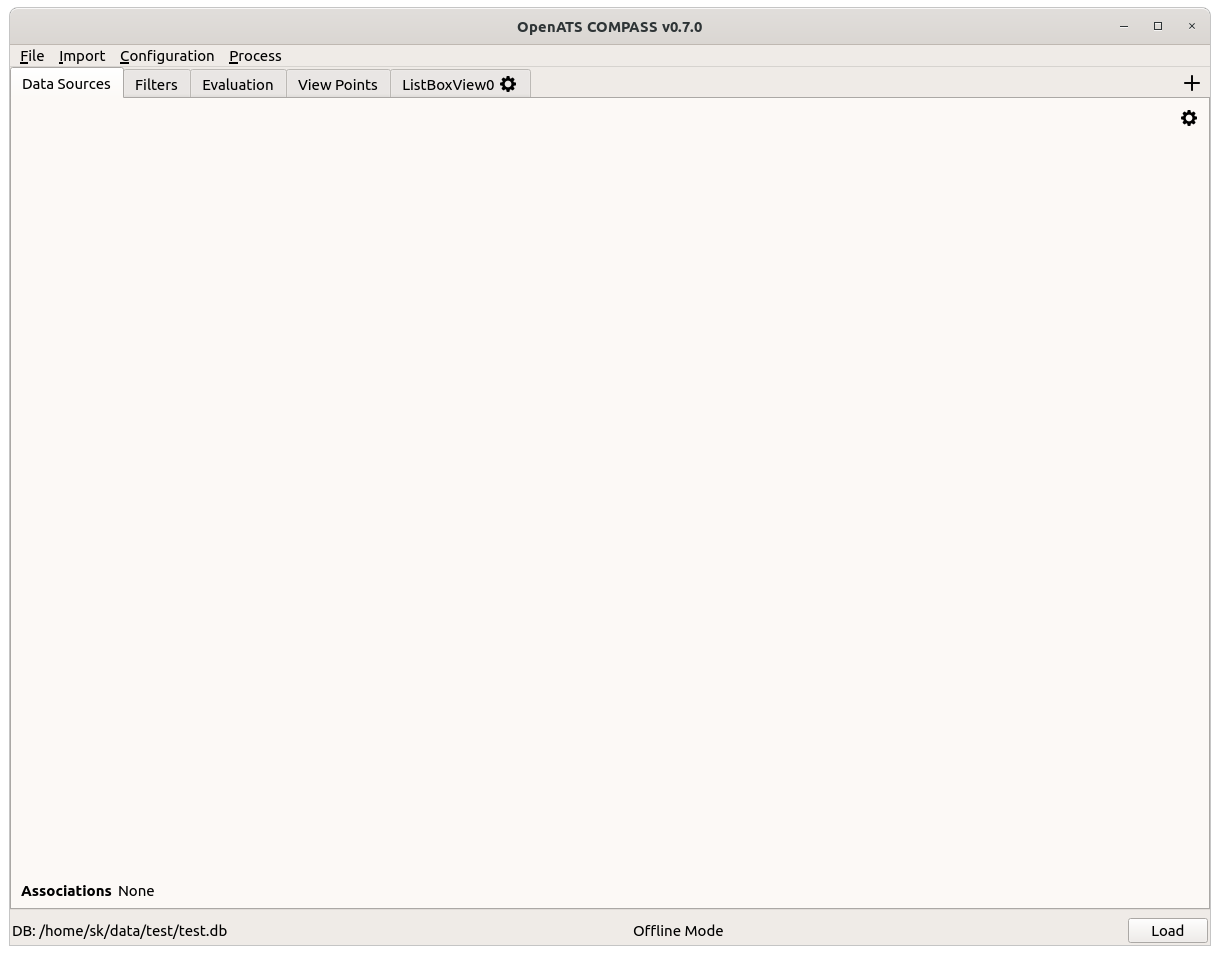
\includegraphics[width=19cm]{figures/main_window_opened.png}
  \caption{Main Window After Opening a Database}
\end{figure}

\subsection{Import Menu}

Databases can be created, opened and closed using the File menu.

\begin{figure}[H]
  \center
    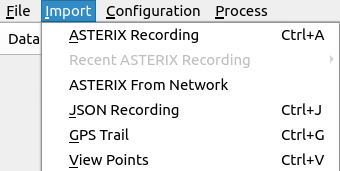
\includegraphics[width=6cm,frame]{figures/ui_import_menu.png}
  \caption{File Menu}
\end{figure}

\begin{itemize}
 \item ASTERIX Recording: Import ASTERIX recording file
 \item Recend ASTERIX Recording: Import recent ASTERIX recording file
 \item ASTERIX From Network: Import ASTERIX from network interfaces in Live mode
 \item GPS Trail: Import (D)GPS trail from NMEA file
 \item View Points: Import View Points definition file
\end{itemize}
\  \\

\subfile{ui_import_data}
\subfile{ui_configuration}
\subfile{ui_postprocess}
\subfile{ui_use_cases}

% \subfile{task_open_database}

% \subfile{task_manage_schema}
% \subfile{task_manage_dbo}

% \subfile{task_import_view_points}
% \subfile{task_import_asterix}
% \subfile{task_import_json}
% \subfile{task_import_mysql}
% \subfile{task_import_gps}

% \subfile{task_manage_datasources}
% \subfile{task_manage_sectors}

% \subfile{task_calc_radar_pos}

% \subfile{task_postprocess}

% \subfile{task_associate_tr}
% \subfile{task_associate_artas_tris}

% \subfile{task_starting}


